\documentclass[11pt]{article}
\usepackage[margin=1in]{geometry}
\usepackage{volfit_preamble}
\graphicspath{{figures/}}

\title{\textbf{Trust Is Computed}\\[2pt]
\large The observation filter as two honest covariances: a gain that is an
output, and an audit in standardized residuals\\[2pt]
\normalsize Vol-Fitter Technical Notes, No.~15}
\author{Vol-Fitter}
\date{\today}

% Note-local notation.
\newcommand{\calL}{\mathcal L}
\newcommand{\calI}{\mathcal I}
\newcommand{\calH}{\mathcal H}

\begin{document}
\maketitle

% Generated numbers.  kalman_trust_tables.tex carries everything unique to
% this edition (gen_kalman_trust.py); backtest numbers are read from the
% stored sweep artifacts, never re-run.  Never retype a generated number.
% Auto-generated by gen_kalman_trust.py — do not edit.
\newcommand{\ktrgainlevel}{0.80}
\newcommand{\ktrgainskew}{0.72}
\newcommand{\ktrgaincurv}{0.027}
\newcommand{\ktrpostlevel}{20.32}
\newcommand{\ktrpostcurv}{0.112}
\newcommand{\ktrcontrarho}{25}
\newcommand{\ktrcontragainclean}{0.73}
\newcommand{\ktrcontragainkink}{0.20}
\newcommand{\ktrcontragainatm}{0.74}
\newcommand{\ktrunitslope}{0.97}
\newcommand{\ktrclampsparse}{0}
\newcommand{\ktrclampnoreg}{2}
\newcommand{\ktrmoveintra}{14}
\newcommand{\ktrmoveovernight}{52}
\newcommand{\ktrmoveweekend}{37}
\newcommand{\ktrcalbestq}{120}
\newcommand{\ktrzcalintra}{1.04}
\newcommand{\ktrzsesintra}{0.95}
\newcommand{\ktrzcalovernight}{0.53}
\newcommand{\ktrzsesovernight}{0.89}
\newcommand{\ktrzcalweekend}{0.23}
\newcommand{\ktrzsesweekend}{0.84}
\newcommand{\ktroffdiagdrag}{20}
\newcommand{\ktrzstdspiketen}{5.16}
\newcommand{\ktrzstdspikethirty}{1.75}
\newcommand{\ktrerrpostspike}{10.5}
\newcommand{\ktrerrmeasspike}{6.7}
\newcommand{\ktrerrpredspike}{47}
\newcommand{\ktrwinspike}{0.38}
\newcommand{\ktrcontrajacspike}{15.8}
\newcommand{\ktrcontrafacspike}{45.9}
\newcommand{\ktrshockjacspike}{38.6}
\newcommand{\ktrshockfacspike}{18.7}
\newcommand{\ktrzstdhighten}{1.43}
\newcommand{\ktrzstdhighthirty}{0.82}
\newcommand{\ktrerrposthigh}{9.2}
\newcommand{\ktrerrmeashigh}{7.7}
\newcommand{\ktrerrpredhigh}{31}
\newcommand{\ktrwinhigh}{0.49}
\newcommand{\ktrcontrajachigh}{10.5}
\newcommand{\ktrcontrafachigh}{29.7}
\newcommand{\ktrshockjachigh}{78.6}
\newcommand{\ktrshockfachigh}{20.2}
\newcommand{\ktrzstdlowten}{1.32}
\newcommand{\ktrzstdlowthirty}{1.05}
\newcommand{\ktrerrpostlow}{5.3}
\newcommand{\ktrerrmeaslow}{4.0}
\newcommand{\ktrerrpredlow}{22}
\newcommand{\ktrwinlow}{0.49}
\newcommand{\ktrcontrajaclow}{6.3}
\newcommand{\ktrcontrafaclow}{21.7}
\newcommand{\ktrshockjaclow}{11.6}
\newcommand{\ktrshockfaclow}{11.9}
\newcommand{\ktrstepstotal}{38\,181}
\newcommand{\ktrshockimprovemin}{3}
\newcommand{\ktrshockimprovemax}{7}
\newcommand{\ktractthinspike}{6.5}
\newcommand{\ktractcontraspike}{9.1}
\newcommand{\ktrovlcontraspike}{12.1}
\newcommand{\ktrrawcontraspike}{7.9}
\newcommand{\ktrovlshockspike}{4.6}
\newcommand{\ktractshockspike}{19.5}
\newcommand{\ktractthinhigh}{4.8}
\newcommand{\ktractcontrahigh}{5.6}
\newcommand{\ktrovlcontrahigh}{10.6}
\newcommand{\ktrrawcontrahigh}{9.8}
\newcommand{\ktrovlshockhigh}{7.9}
\newcommand{\ktractshockhigh}{25.2}
\newcommand{\ktractthinlow}{3.4}
\newcommand{\ktractcontralow}{4.5}
\newcommand{\ktrovlcontralow}{6.3}
\newcommand{\ktrrawcontralow}{5.4}
\newcommand{\ktrovlshocklow}{4.9}
\newcommand{\ktractshocklow}{6.4}
\newcommand{\ktrstepsvtwo}{39\,190}
\newcommand{\ktractzetamin}{0.4}
\newcommand{\ktractzetamax}{1.4}
\newcommand{\ktrrefagree}{\ensuremath{1.0\times10^{-17}}}
\newcommand{\ktrblowupminpts}{3}
\newcommand{\ktrblowupmaxpts}{28}
\newcommand{\ktreempost}{4.5}
\newcommand{\ktreemmeas}{8.1}
\newcommand{\ktreemzeta}{0.14}
\newcommand{\ktrefazeta}{0.26}
\newcommand{\ktrsglshockwinbefore}{0.42}
\newcommand{\ktrsglshockwinafter}{1.00}
\newcommand{\ktrsglzetabefore}{3.8}
\newcommand{\ktrsglzetaafter}{0.8}
\newcommand{\ktrgencommit}{ccdf6ed}
\newcommand{\ktrgendate}{2026-07-19}


\begin{abstract}
Every fitter that carries state through time owns a dial marked
\emph{trust}: how far should this morning's noisy quotes move yesterday's
surface?  This lecture develops the Vol-Fitter's observation filter from
one design decision --- \emph{the desk never touches that dial}.  The gain
that moves a smile handle toward the market is the ratio of two
covariances, each built honestly from first principles: a measurement
covariance propagated from the fit's own information in \emph{stated}
noise units (bid--ask half-spreads --- double the stated noise, quadruple
the covariance, measured slope \ktrunitslope), inflated by realized
inconsistency (a two-strike contradiction drives the inflation to its cap
of \ktrcontrarho\ and turns the curvature gain from \ktrcontragainclean\
down to \ktrcontragainkink\ with nobody touching anything); and a
prediction covariance grown by a process clock that must itself be honest
--- on stored thirty-minute data a weekend moves the ATM no more than one
overnight (\ktrmoveweekend\ vs \ktrmoveovernight\ bp), so no calendar
clock calibrates all cadences and the shipped session clock does.  The
acceptance test is never smoothness: it is whether the standardized
residuals $\zeta$ have unit scale --- error bars that mean what they say.
By that audit a \ktrstepstotal-step temporal backtest flipped the clock
noise default ($10\to30$ bp$/\sqrt{\text{day}}$: $\zeta$ std
\ktrzstdspiketen$\,\to\,$\ktrzstdspikethirty\ in the spike regime), chose
the Jacobian covariance route ($2$--$3\times$ better contradiction
rejection), and convicted the full-covariance update (off-diagonal gains
dragged the ATM through junk curvature by
\ktrblowupminpts--\ktrblowupmaxpts\ vol points on coarse chains; production
updates per handle).  A second \ktrstepsvtwo-step sweep scored the active
one-stage MAP --- the same accounting done inside the objective --- as the
best denoiser wherever denoising is the job, and its shock lag as the cost
of a prior priced before the measurement exists; the shipped answer
(a fit-free ATM probe plus one-step-lagged gating) closes that gap by
construction and awaits its full-regime validation.
\end{abstract}

\newpage
\tableofcontents
\newpage

%======================================================================
\section{The dial nobody may own}
\label{sec:dial}

Two mornings, two failures.  On the first, a dense at-the-money cluster
contains one stale strike: chase the mids literally and the fit grows a
curvature kink that no one traded.  On the second, the whole chain
genuinely reprices overnight: hold on to yesterday and the book carries a
stale surface into a moved market.  A fitter that persists state must
steer between these, and the tempting instrument is a slider --- ``how
much do we trust this morning?'' --- tuned by hand, per desk, per mood.

The Vol-Fitter refuses the slider.  In one dimension the whole machinery
of this note is the identity
\[
m^{+}=\frac{r}{p+r}\,m^{-}+\frac{p}{p+r}\,z ,
\]
the posterior as a precision-weighted average of the predicted handle
$m^-$ (variance $p$) and the observed handle $z$ (variance $r$).  The
weight $K=p/(p+r)$ --- the Kalman gain --- is not a setting.  It is an
\emph{output}, computed from two uncertainty budgets, and every design
decision in the feature is about making those two budgets tell the truth:
$r$ must reflect what the quotes actually pin down, in the market's own
noise units; $p$ must reflect how much the smile can genuinely have
diffused, on the clock the market actually runs on.  When both are
honest, the dial turns itself: the stale-strike kink arrives with a large
$r$ and is barely admitted; the genuine reprice arrives with a large
innovation, widens $p$ through a gated surprise term, and is followed.

\begin{heuristic}
This note and Note~13 divide the world by \emph{sufficient statistic}.
Prior persistence asks ``where did the market not speak?''\ and acts
through a gap gate that is exactly zero where quotes identify a feature.
The filter asks ``the market spoke here --- how noisy was its voice?''\
and acts through a covariance that is never zero and never infinite.  A
sparse wing is a gap: persistence fills it.  A dense-but-contradictory
cluster is a noisy observation: the filter shrinks it.  Confusing the two
is the classic failure this pair of notes exists to prevent.
\end{heuristic}

\begin{invariant}
\begin{enumerate}[leftmargin=1.6em]
\item Trust enters the update only through an explicit prediction
covariance and an explicit measurement covariance --- never through a
hand-set weight on either side.
\item The same quote is never counted twice: once a posterior exists, it
may not be re-anchored against the quotes that built it
(\cref{prop:nodouble}).
\item The filter state is an arbitrage-safe coordinate --- the exact ATM
handles of Note~01 --- never a free raw-IV curve and never native
local-vol parameters.
\item Mode \texttt{off} is byte-identical to the feature never existing,
and every filter call on the fit path is advisory: a filter failure
cannot break a calibration.
\item Every filtered output reports prediction, observation, innovation,
gain and posterior uncertainty --- the full audit, per handle, per step.
\item Prior persistence continues to act only on functionals the current
market does not identify; the filter never touches them.
\end{enumerate}
\end{invariant}

\paragraph{Conventions and the notation ledger.}
One time symbol, $\tau$, the node's variance time; $\Delta t$ is the
elapsed process-noise time between snapshots (whose \emph{clock} is
\cref{sec:clock}'s subject) and $h=\log(F_t/F_{t-1})$ the log-forward
move.  Subscripted $\partial$ for the rare partial derivative; primes are
never used.

\begin{table}[H]
\centering\footnotesize
\setlength{\tabcolsep}{3pt}
\begin{tabular}{@{}llll@{}}
\toprule
$x=(\sigma_{\atm},s,\kappa)\T$ & the handle state &
$m^{\mp},\,P^{\mp}$ & prediction / posterior law\\[2pt]
$z,\ R$ & handle observation and its covariance &
$K,\ S,\ \nu$ & gain; innovation covariance; innovation\\[2pt]
$Q,\ q$ & process covariance; its ATM clock scale &
$J,\ G,\ \calI_\theta$ & solver / handle Jacobians; information\\[2pt]
$\rho,\ \chi^2$ & residual inflation; quote misfit &
$s_q$ & stated per-quote noise std (vol units)\\[2pt]
$\zeta$ & standardized residual &
$\Delta t,\ h,\ \tau$ & elapsed time; forward move; variance time\\
\bottomrule
\end{tabular}
\caption{Every symbol in the note.  $\calH$ extracts handles from a
model, $\calL$ names a loss; nothing is reused with a second meaning.}
\label{tab:ledger}
\end{table}

The state deserves its sentence.  $x_t$ is the compact handle vector
(ATM vol, ATM skew, ATM curvature) --- the same three coordinates the
graph extrapolator of Note~14 propagates, read exactly off the LQD
backbone (Note~01), so the filtered object is arbitrage-safe by
construction and model-agnostic by carrier (signed operators such as
RR25/BF25 are a dimension-agnostic extension left for after the pilot).
Raw option mids are a poor state space --- contracts appear and
disappear, the OTM side flips with the forward, American quotes need
de-Americanization, and a smoothed raw-IV vector is not guaranteed
butterfly-free --- so the filter begins \emph{after} the quote-prep
pipeline, and its measurement is a fit, not a quote vector
(\cref{sec:robs}).

%======================================================================
\section{The update that survives any gain}
\label{sec:update}

\begin{definition}[Predicted and observed handle laws]
\label{def:laws}
At snapshot $t$, with $\mathcal F_{t-1}$ the filtration of previous
snapshots,
\[
x_t\given\mathcal F_{t-1}\sim\mathcal N(m_t^-,P_t^-),
\qquad
z_t\given x_t\sim\mathcal N(H_t x_t,R_t),
\]
where $m_t^-$ is the transported previous filtered state
(\cref{sec:pbudget}), $z_t$ and $R_t$ are extracted from today's prepared
quotes without any temporal prior (\cref{sec:robs}), and $H_t$ is the
measurement operator ($I$ for a direct handle observation; the equations
allow a subset or a linear functional).
\end{definition}

The update is the covariance-form Kalman step in Joseph form:
\begin{equation}
\boxed{\;
\begin{aligned}
S_t&=H_tP_t^-H_t\T+R_t,\\
K_t&=P_t^-H_t\T S_t^{-1},\\
m_t^+&=m_t^-+K_t\big(z_t-H_tm_t^-\big),\\
P_t^+&=(I-K_tH_t)P_t^-(I-K_tH_t)\T+K_tR_tK_t\T .
\end{aligned}
\;}
\label{eq:kalman}
\end{equation}

The last line is longer than the textbook $P^+=(I-KH)P^-$, and the extra
length is the point: the Joseph form is a \emph{sum of two sandwiches},
symmetric and positive semidefinite for \emph{any} gain matrix, optimal
or not.  That algebraic fact is a design asset.  It makes the pilot's
own-gain cap safe (a capped $K$ is a valid, merely suboptimal, linear
gain whose posterior covariance is still a covariance), and it makes the
diagonalized update of \cref{sec:matrix} safe for the same reason.  The
production body is small enough to quote whole:

\begin{lstlisting}[caption={The production update (quoted from
\texttt{calib/observation\_filter.py}): \cref{eq:kalman} with the
own-gain pilot cap, Joseph covariance, and an explicit PSD guard.
Verified against the reference listing of \cref{app:ref} to
\ktrrefagree.},label={lst:crux}]
innovation = z - H @ m
S = H @ P @ H.T + R
K = np.linalg.solve(S.T, (P @ H.T).T).T   # gain without an explicit inverse
if max_gain < 1.0:                        # pilot cap: scales OWN-gains only
    own = np.abs(np.diag(K @ H))
    scale = np.minimum(1.0, max_gain / np.maximum(own, 1e-300))
    K = K * scale[:, None]
out_mean = m + K @ innovation
i_kh = np.eye(m.size) - K @ H
out_cov = i_kh @ P @ i_kh.T + K @ R @ K.T # Joseph form: PSD for ANY gain
out_cov = 0.5 * (out_cov + out_cov.T)
if np.any(np.linalg.eigvalsh(out_cov) < -1e-12):
    raise FloatingPointError("posterior covariance lost PSD")
\end{lstlisting}

\begin{proposition}[Precision-weighted shrinkage]
\label{prop:scalar}
In one dimension with $H=1$, prediction variance $p$ and measurement
variance $r$,
\[
m^+=\frac{r}{p+r}\,m^-+\frac{p}{p+r}\,z,
\qquad K=\frac{p}{p+r}\in(0,1),
\]
so the posterior always lies strictly between prediction and
observation, and moves toward whichever carries the smaller stated
variance.
\end{proposition}

\begin{proof}
$S=p+r$ and $K=p/S$; substitute into $m^+=m^-+K(z-m^-)$.  Positivity of
$p$ and $r$ places $K$ in $(0,1)$.
\end{proof}

\Cref{fig:case} runs the note's canonical vignette through the
production update.  The transported prediction says
$(20.0\%,-0.35,0.10)$ with standard deviations $(0.30\%,0.08,0.05)$;
today's data-only fit reads $(20.4\%,-0.37,0.55)$ --- a plausible level
move, a plausible skew, and a curvature kink manufactured by one stale
close strike.  The measurement builder of \cref{sec:robs} prices that
chain at $\sqrt{\diag R}=(0.15\%,0.05,0.30)$: level and skew tight,
curvature wide because the cluster contradicts itself.  The computed
gains follow: $K_\sigma=\ktrgainlevel$, $K_s=\ktrgainskew$,
$K_\kappa=\ktrgaincurv$.  The posterior tracks the market's level to
$\ktrpostlevel\%$ and accepts $2.7\%$ of the kink
($m^+_\kappa=\ktrpostcurv$) --- not vetoed, priced.  No gap logic fired:
by quote count this region is superbly observed, which is exactly why
Note~13's gate must stay closed and the covariance must do the work.

\begin{figure}[H]
\centering
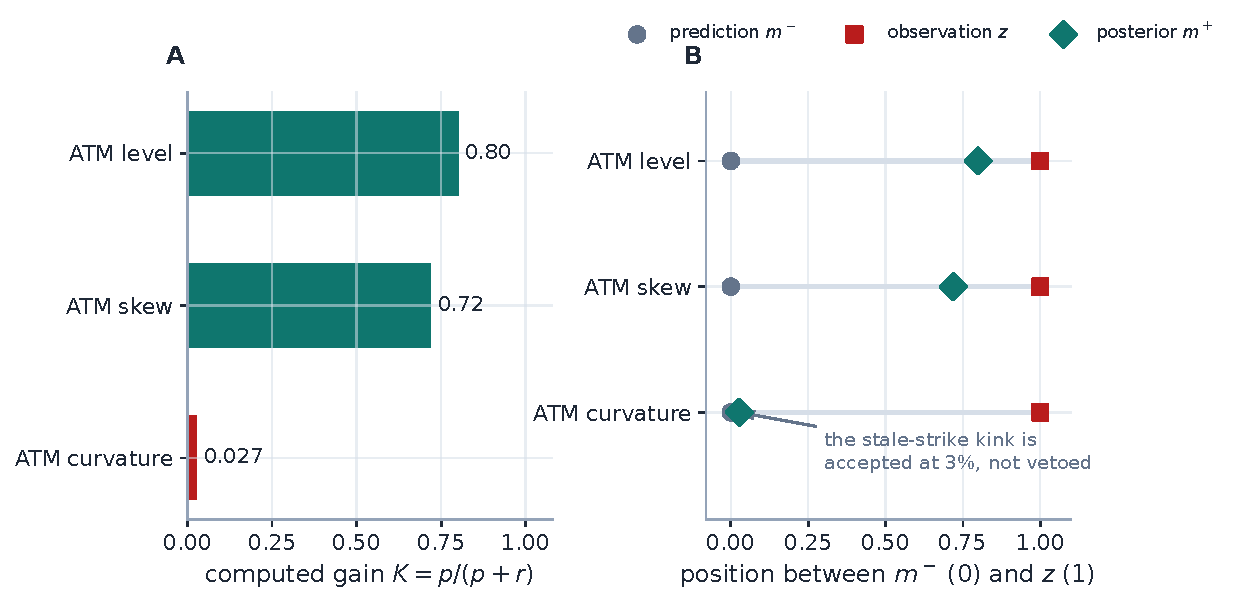
\includegraphics[width=\textwidth]{fig_ktr_case.pdf}
\caption{The case file through the production update.  A: the computed
per-handle gains --- level and skew admitted at \ktrgainlevel\ and
\ktrgainskew, the contradiction-inflated curvature at \ktrgaincurv.
B: each posterior lands on the prediction$\to$observation segment
exactly at its gain: in the normalized coordinate the position \emph{is}
the gain, so the reader can check \cref{prop:scalar} by eye.}
\label{fig:case}
\end{figure}

\paragraph{Exercise 1.}
Show that the Joseph form in \cref{eq:kalman} equals
$P^- - K S K\T$ at the optimal gain, but remains PSD for any $K$
(write it as $A P^- A\T + K R K\T$ with $A=I-KH$).  Then show the
textbook form $(I-KH)P^-$ loses symmetry --- and can lose positivity ---
the moment $K$ is perturbed, e.g.\ by the own-gain cap of
\cref{lst:crux}.  The cap is safe \emph{because} production pays for the
longer formula.

%======================================================================
\section{The observation budget: what did the market actually say?}
\label{sec:robs}

The Kalman algebra is a page; the work is the covariance.  $R_t$ must
answer, in vol units, ``how precisely do today's quotes pin each
handle?''\ --- and it must answer honestly on chains that are sparse,
wide, stale, or self-contradictory.  Production builds it in four moves.

\subsection{A fit is the observation}

The extractor is a two-step map,
\begin{equation}
z_t=\calH\Big(\argmin_\theta\
\calL_{\mathrm{quote}}(\theta;q_t)+\calL_{\mathrm{intrinsic}}(\theta)\Big),
\label{eq:extract}
\end{equation}
where $\calL_{\mathrm{quote}}$ is the vega-normalized, bid--ask-aware
loss of Note~07, $\calL_{\mathrm{intrinsic}}$ contains only the model
regularization needed for a valid no-arbitrage smile (never temporal
persistence), and $\calH$ reads the exact ATM handles off the fitted
slice.  The carrier is the LQD backbone --- always fitted,
model-agnostic, closed-form handles --- so $z_t$ costs nothing extra.
When the committed fit did receive persistence targets (hybrid mode with
an active prior), the measurement is flagged \texttt{contaminated}
rather than silently trusted; Note~13's gate keeps the overlap near zero
exactly where the filter has signal, and the opt-in
\texttt{filterDataOnlyPrepass} buys a strictly clean $z_t$ for one extra
data-only fit per node.

\subsection{Information, in stated noise}
\label{sec:units}

Near the optimum, linearize the residual stack $r(\theta)\approx
r(\hat\theta)+J(\theta-\hat\theta)$; with the handle map $x=g(\theta)$
and its Jacobian $G$, the delta method gives the default (Jacobian)
route:
\begin{equation}
\calI_\theta=J\T WJ+\Lambda_{\mathrm{intrinsic}},
\qquad
R_x\approx G\,\calI_\theta\pinv\,G\T .
\label{eq:cov-delta}
\end{equation}
Every calibrator retains its solution Jacobian in a diagnostics
side-channel with the square-root weights and inverse-vega scaling
already folded in, so $J\T J$ \emph{is} the observed information in vol
units and the intrinsic rows (ridge, calendar, barrier) supply
$\Lambda_{\mathrm{intrinsic}}$ automatically; $G$ is a central finite
difference of the handle map --- slice \emph{builds}, not fits, on the
coarse optimization grid.

\begin{caution}
Information is only information \emph{in stated noise}.  The production
quote weights are relative (equal or time-value density, Note~07), not
$1/\text{noise}^2$; read at face value, $J\T WJ$ is the information
under an implied noise of one full volatility point per quote --- so
small that $R_x$ saturates every sanity envelope and the filter freezes.
The shipped builder fixes the units at the source: the data rows of $J$
and $r$ are divided by the stated per-quote noise standard deviation
$s_q$ --- the bid--ask half-spread floored at one vol bp, or the haircut
--- \emph{before} the information and $\chi^2$ are formed, while the
intrinsic rows keep their own scale (they are a prior, not a
measurement).  $R_t$ then obeys the quadratic contract the algebra
assumes, and \cref{fig:units}A measures it: log-slope \ktrunitslope\
of $\sqrt{R_{\sigma\sigma}}$ in $s_q$ --- double the stated noise,
quadruple the covariance.  The same $s_q$ reappears twice in active mode
(\cref{sec:map}): in the MAP prior weights and in the posterior
unwhitening --- one consistent value in both places, or the MAP algebra
silently breaks.
\end{caution}

The pseudo-inverse in \cref{eq:cov-delta} is deliberately a
\emph{regularized} eigen-inverse: eigenvalues of $\calI_\theta$ below
$10^{-10}\lambda_{\max}$ are clamped \emph{up} to the cutoff, so a
$\theta$-direction the quotes do not identify contributes a
large-but-finite handle variance.  The sign of this failure mode is the
whole point.  A strict pseudo-inverse zeroes small eigenvalues --- and
thereby reports an \emph{unidentified} direction as \emph{zero}
uncertainty, the one lie a filter must never inherit from its
measurement.  On production chains the intrinsic rows usually keep
$\calI_\theta$ numerically full-rank (\cref{fig:units}B: zero clamped
directions even at five quotes, while $\sqrt{R_{\kappa\kappa}}$ grows
threefold); strip them and the clamp fires (\ktrclampnoreg\ directions
on the five-quote chain) --- the last fence, behind the fence that
usually holds.

\begin{figure}[H]
\centering
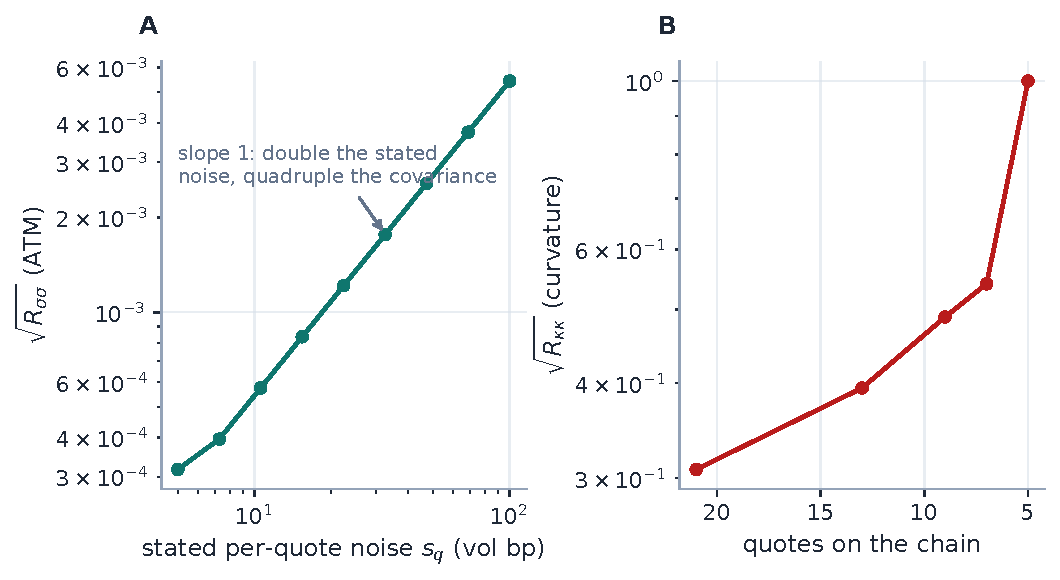
\includegraphics[width=\textwidth]{fig_ktr_units.pdf}
\caption{The two unit disciplines of the observation budget (production
builder throughout).  A: the quadratic contract --- the ATM measurement
std against the stated per-quote noise has log-slope \ktrunitslope;
covariance is stated noise squared, propagated, not a house opinion.
B: thinning the chain from 21 quotes to 5 triples the curvature
uncertainty \emph{finitely}: the intrinsic rows keep the information
full-rank (zero clamped directions), and the eigen-clamp stands behind
them for the day they do not.}
\label{fig:units}
\end{figure}

\subsection{Contradiction is noise: the $\chi^2$ inflation}
\label{sec:inflation}

The covariance so far measures \emph{geometry} --- which directions the
quote locations identify.  It does not yet know whether the quotes agree
with each other.  That enters through realized inconsistency:
\begin{equation}
R_t=\rho_t\,R_x,\qquad
\rho_t=\operatorname{clip}\!\left(\frac{\chi_t^2}{\max(m-d,1)},\,1,\,
25\right),
\qquad
\chi_t^2=r(\hat\theta)\T W r(\hat\theta)\ \text{(quote rows only)},
\label{eq:resid-inflation}
\end{equation}
with $m$ the quote count, $d$ the handle count, and the cap preventing
one broken chain from poisoning the state.  A dense cluster that cannot
be fitted within its stated noise is not well-observed --- it is loud
and wrong, and $\rho_t$ says so.

\Cref{fig:contra} is the mechanism figure of the note.  A clean
21-quote chain is progressively contradicted: two adjacent strikes are
kinked in opposite directions by up to three vol points (the temporal
backtest's \texttt{contradiction} scenario).  The production pipeline
responds exactly as designed: $\chi^2$ grows, $\rho$ climbs from $1$ to
its cap of \ktrcontrarho, the stated curvature noise triples to the
sanity envelope, and the computed curvature gain falls from
\ktrcontragainclean\ to \ktrcontragainkink\ while the ATM gain --- whose
direction the kink barely pollutes --- stays at \ktrcontragainatm.  No
threshold, no veto, no knob: the misfit turned the dial.

\begin{figure}[H]
\centering
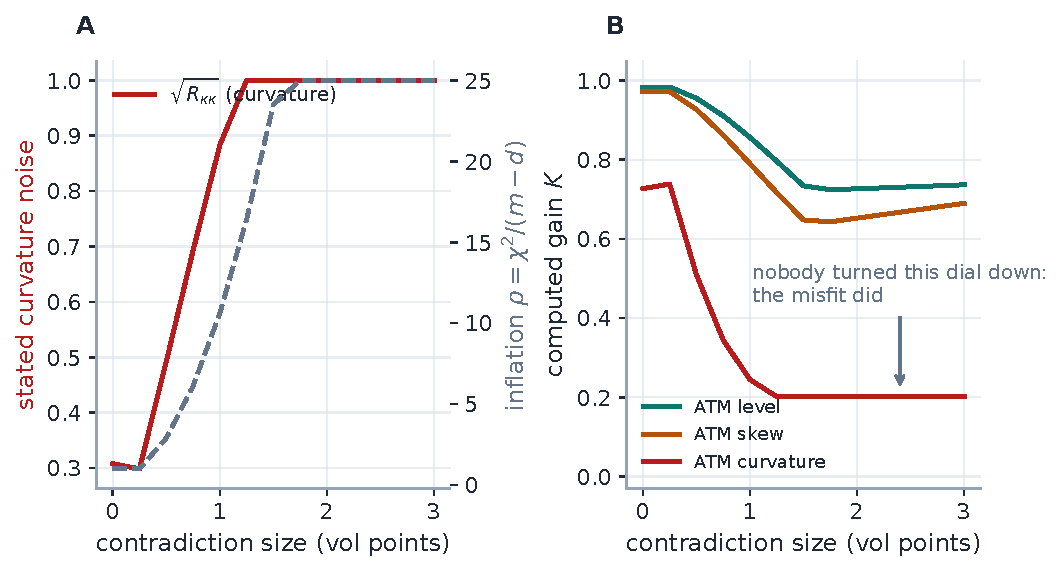
\includegraphics[width=\textwidth]{fig_ktr_contra.pdf}
\caption{A contradiction prices itself (production fit, measurement
builder and update; two adjacent strikes kinked $\pm\varepsilon$).
A: the realized-misfit inflation $\rho$ climbs to its cap of
\ktrcontrarho\ and the stated curvature noise rises to the envelope.
B: the computed gains respond --- curvature from \ktrcontragainclean\
to \ktrcontragainkink, the better-identified level and skew far less.
The flat tails are the caps: beyond them the chain is already maximally
distrusted.}
\label{fig:contra}
\end{figure}

\begin{remark}[Bid--ask bands come for free]
In band mode, quotes inside the spread should not pretend to identify
the mid.  On the Jacobian route no special-casing is needed: inactive
hinge rows differentiate to zero inside the spread, so in-band quotes
contribute nothing to $J\T WJ$ and only the weak mid anchor remains.
This matches Note~07's semantics --- inside the spread the market is a
set, not a point --- and is a concrete advantage over the factor route,
which must proxy band width through a scalar spread factor.
\end{remark}

\subsection{The fallback route, and the short-dated floor}

When no solution Jacobian was retained (cached fits), a cheaper builder
reuses the graph layer's precision vocabulary,
\begin{equation}
R_t^{-1}
=\diag(c_h)\,\pi_{\mathrm{fit}}\,
f_{\mathrm{density}}\,f_{\mathrm{spread}}\,f_{\mathrm{fresh}},
\label{eq:cheapR}
\end{equation}
with per-handle confidences $c_h$, inverse squared fit RMS (floored and
capped), and the shared scalar factors of Note~13.  The realized misfit
already lives in the RMS factor, so no separate $\rho$ is applied ---
it would double-count.  This route also survives as the sweep's A/B
column, which is how the Jacobian route's advantage got \emph{measured}
rather than assumed (\cref{sec:audit}).

One more honesty term, measured before it was priced: below $30$ days
to expiry the thinned-vs-full ATM discrepancy runs $2$--$3\times$ the
stated half-spread (short-end quote and de-Americanization noise --- the
Note~04/05 diagnosis, not a filter defect).  The stated noise is
therefore scaled by $\sqrt{30\,\mathrm{DTE}/\mathrm{DTE}}$ below $30$
DTE (never below one), applied consistently to $R_t$, the active MAP
weights and the posterior unwhitening.

\begin{example}[title={Case file: close-strike contradiction versus true
gap}]
\textbf{Setup.}  A one-month smile: nine near-ATM quotes, nothing
reliable beyond $25\Delta$, one stale close strike forcing a large
curvature if mids are chased --- the market of \cref{fig:case}.

\textbf{Diagnosis.}  Quote density says the ATM region is superbly
observed, so Note~13's activation gate is closed there --- using
persistence to pull the curvature back would damp with yesterday what
should be judged by today.  The contradiction instead surfaces as
measurement noise through \cref{eq:resid-inflation}, and the computed
gains split the day correctly: level \ktrgainlevel, skew \ktrgainskew,
curvature \ktrgaincurv.

\textbf{Persistence.}  The unquoted wing is the opposite case:
observation precision below requirement, gate open, transported prior
holding the tail.  The same morning legitimately carries both
mechanisms, each on its own sufficient statistic.

\textbf{The other half.}  A rejected kink must not become a rejected
\emph{move}: when the whole chain genuinely reprices, the innovation is
coherent across handles, the surprise gate of \cref{sec:pbudget} widens
$P^-$, and the filter follows the market.  \emph{A dense cluster with a
bad internal residual is a high-$R$ observation; a strike range with no
reliable quotes is a gap.  The first belongs to the filter, the second
to persistence.}
\end{example}

%======================================================================
\section{The prediction budget: how far can the smile have walked?}
\label{sec:pbudget}

The other covariance is the prediction's.  The previous filtered state
is transported to today --- mean by the spot-vol rules of Note~12,
uncertainty by a process budget:
\begin{equation}
m_t^-=\mathcal T_t(m_{t-1}^+),
\qquad
P_t^-=P_{t-1}^++Q_t,
\qquad
Q_t=Q_{\mathrm{clock}}+Q_{\mathrm{spot}}
+Q_{\mathrm{event}}+Q_{\mathrm{source}}+Q_{\mathrm{model}} .
\label{eq:transport}
\end{equation}
The mean transport is the first-order handle map of the SSR transport
(Note~12): for a log-forward move $h$,
\begin{equation}
\sigma_{\atm}\mapsto\sigma_{\atm}+\mathrm{SSR}\cdot s\,h,
\qquad
s\mapsto s+\kappa\,h,
\qquad
\kappa\mapsto\kappa,
\label{eq:transport-handles}
\end{equation}
with the transport Jacobian deferred ($A_t=I$; a full curve transport is
not available for a bare handle vector, and seeding uses the exact curve
transport through the prior machinery instead) --- the uncertainty
growth is carried entirely by $Q$.  Its terms: a clock term
$q^2\,\Delta t$ per handle (the headline knob, in vol bp per
$\sqrt{\text{day}}$); a spot-transport term with std proportional to
$\abs h$ in each handle's typical move scale (the same intuition as
persistence's transport-distance factor); and event, source and model
widenings supplied by the app layer when the prediction crosses an event
window, a provider or as-of switch, or a display-model change.

\begin{caution}
Do not filter native local-vol parameters.  The local-vol grid
(Note~04) is a projection machinery with its own PDE stability and
no-arbitrage constraints; filter the target smile handles, then project
or refit the surface to the filtered target.
\end{caution}

\subsection{The clock the variance actually runs on}
\label{sec:clock}

$Q_{\mathrm{clock}}=q^2\Delta t$ looks innocent until one asks what
$\Delta t$ \emph{is}.  The design note ran on calendar days; Note~11
already warned that the market keeps its own clock, and the stored
thirty-minute campaign (three tickers, eight days spanning the July-4th
closure) measures the failure directly.  On those tables the median
absolute ATM move is \ktrmoveintra\ bp per thirty-minute session step,
\ktrmoveovernight\ bp across one overnight --- and \ktrmoveweekend\ bp
across the entire three-day holiday closure.  \emph{A closed market
adds nothing an overnight does not already contain.}  A calendar clock
must therefore be wrong at some cadence: whatever $q$ it picks, it pays
three-plus days of variance across a closure that delivers one
overnight's worth.  The audit shows exactly that
(\cref{fig:clock}B): the best calendar configuration
($q=\ktrcalbestq$ bp) is calibrated intraday
($\zeta$ std \ktrzcalintra) but overdispersed into closures
($\zeta$ std \ktrzcalovernight\ overnight, \ktrzcalweekend\ across the
weekend --- error bars three and four times too wide).  The shipped
session clock --- $60\%$ of a day's variance in the exchange
session, closed days at weight zero, the intraday variance clock of the
0DTE machinery --- calibrates all three cadences at once
($\zeta$ std \ktrzsesintra/\ktrzsesovernight/\ktrzsesweekend\ at
$q=90$ bp).  The default remains \texttt{calendar} (byte-identical to
the pre-clock filter; the session clock is the sub-day workflow's
setting), and the \emph{reset} rule deliberately stays on calendar
hours: staleness is about data age, not variance accrual.

\begin{figure}[H]
\centering
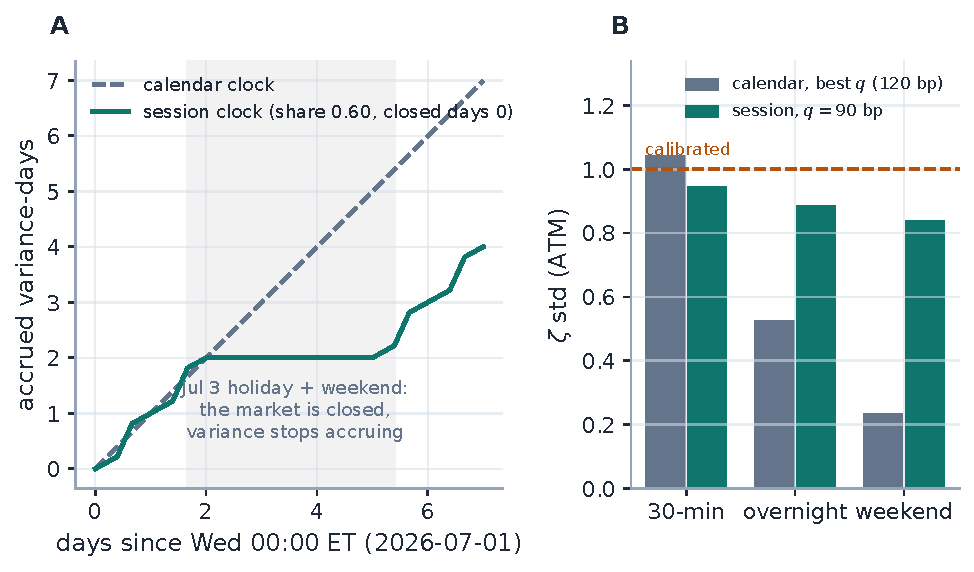
\includegraphics[width=\textwidth]{fig_ktr_clock.pdf}
\caption{The prediction budget runs on the market's clock (production
intraday variance clock; stored 0DTE campaign artifacts).  A: accrued
variance-days across the July-4th week --- the calendar clock pays
through the three-day closure; the session clock (share $0.60$, closed
days $0$) stops, because measured smiles do too.  B: the consequence in
the audit currency: no calendar $q$ is calibrated at every cadence ---
the best one is right intraday and $3$--$4\times$ overdispersed into
closures --- while the session clock at $q=90$ bp holds $\zeta$ std near
$1$ across all three.}
\label{fig:clock}
\end{figure}

\subsection{Surprise must widen the budget: the adaptive gate}
\label{sec:adaptive}

A fixed clock cannot span calm and spike regimes: a genuine five-point
overnight jump is ${\sim}50\sigma$ under a $30$ bp$/\sqrt{\text{day}}$
prior, and a filter that believes its budget lags it.  The shipped
answer is an innovation-gated widening: per handle, when the
standardized innovation $\abs\nu/\sqrt{P^-+R}$ exceeds the gate
(default $3$), $P^-$ is inflated by $(\zeta/3)^2$, capped, so the
surprise reads as ${\sim}3\sigma$ and the gain rises toward the data.
Two properties make it safe.  Clean days never trip it --- below the
gate the update is byte-identical.  And a \emph{contradictory} chain
does not trip it either: its $\rho$-inflated $R$ already shrinks the
standardized innovation, so junk is not chased --- the two honesty
mechanisms compose.  Measured on the spike fixtures: shock win rate
\ktrsglshockwinbefore$\,\to\,$\ktrsglshockwinafter\ with $\zeta$ std
\ktrsglzetabefore$\,\to\,$\ktrsglzetaafter, clean days unchanged; the
full-scale validation is \cref{sec:audit}'s.

\subsection{Seeding, resets, and what survives a recalibration}
\label{sec:lifecycle}

A filter is only as trustworthy as its life-cycle rules.  Seeding: with
a saved prior snapshot, the first state is the \emph{transported} prior
through Note~13's provenance hierarchy at provenance-tier covariance;
without one, the committed fit's own backbone handles at bootstrap-tier
precision --- the same information a bootstrap fetch would produce, for
free, and deliberately \emph{never} a hidden extra fit
(\cref{app:perf} records the incident that made this a rule).  Resets:
a manual quote edit moves the session version and resets the node (the
edited chain invalidates the measurement the state was built on); a
calendar gap beyond \texttt{filterResetHours} resets as \texttt{stale}
(predicting across a long dark period is worse than reseeding); a source
or as-of change wipes the store outright --- a live stream and a
prior-close snapshot are not the same stochastic clock.  Every reset
records its reason.  And recalibration keeps the state: the update is
sequential, one step per genuinely \emph{new} observation, idempotent
per (node, data version, session version) --- recalibrating an unchanged
snapshot re-reads the stored state; a refetch is a new observation, not
a reset.

%======================================================================
\section{When trust is a matrix}
\label{sec:matrix}

Everything so far reads naturally per handle.  The design allowed more:
a full $3\times3$ update, whose off-diagonal gains let one handle's
innovation move another's posterior.  That is not a bug --- it is the
optimal estimator when the stated correlations are true.  The backtest's
second case file is what happens when they are not quite true enough to
spend.

\begin{example}[title={Case file: the off-diagonal blow-up on coarse
chains}]
\textbf{Setup.}  The Phase-5 temporal backtest replayed the August 2024
spike pair across the eight pilot assets in overlay mode ---
full-covariance update, Jacobian route, \cref{eq:kalman} verbatim.

\textbf{Failure mode.}  On EEM and EFA --- coarse-strike, wide-spread
ETF chains --- the posterior ATM error reached
\ktrblowupminpts--\ktrblowupmaxpts\ \emph{vol points}, worse than
\emph{both} baselines.  A scalar update cannot do that:
\cref{prop:scalar} pins its posterior between prediction and
observation.  The damage had to be cross-handle.

\textbf{Diagnosis.}  On a coarse chain few strikes identify level and
curvature separately, so the Jacobian covariance carries strong
level--curvature correlation; a junk curvature innovation then drags
the ATM level through the off-diagonal entries of $K$.
\Cref{fig:offdiag} reproduces the mechanism in vitro with the
production update: a pure curvature innovation against a
correlation-$0.95$ measurement moves the ATM posterior by
\ktroffdiagdrag\ vol bp while the diagonalized update, fed the same
numbers, moves it not at all.  The pilot gain cap is no defence:
\texttt{filterMaxGain} caps the \emph{own}-gains $\diag(KH)$, and the
drag travels through terms it never touches.

\textbf{Fix.}  Production diagonalizes $P^-$ and $R$ before the update
--- per-handle scalar gains, the Note~14 graph convention.  The Joseph
form makes the diagonalized gain \emph{valid} (\cref{sec:update}); the
measured incident is what makes it \emph{right}: the off-diagonals of
trust must themselves be trusted, and on coarse chains the estimated
correlations are exactly the least reliable numbers in the covariance.
The full update remains available for later study --- the correlations
are real information, and a shrunk-correlation update is a live research
item, not a closed door.

\textbf{Verdict.}  Post-fix, EEM wins against the raw measurement
(\ktreempost\ vs \ktreemmeas\ bp, $\zeta$ mean \ktreemzeta) and EFA
degrades gracefully --- near-zero gain from its wide-spread $R$,
$\zeta$ mean \ktrefazeta: conservative rather than wrong.
\emph{An honest one-dimensional trust ledger beats a three-dimensional
one with unreliable cross-entries.}
\end{example}

\begin{figure}[H]
\centering
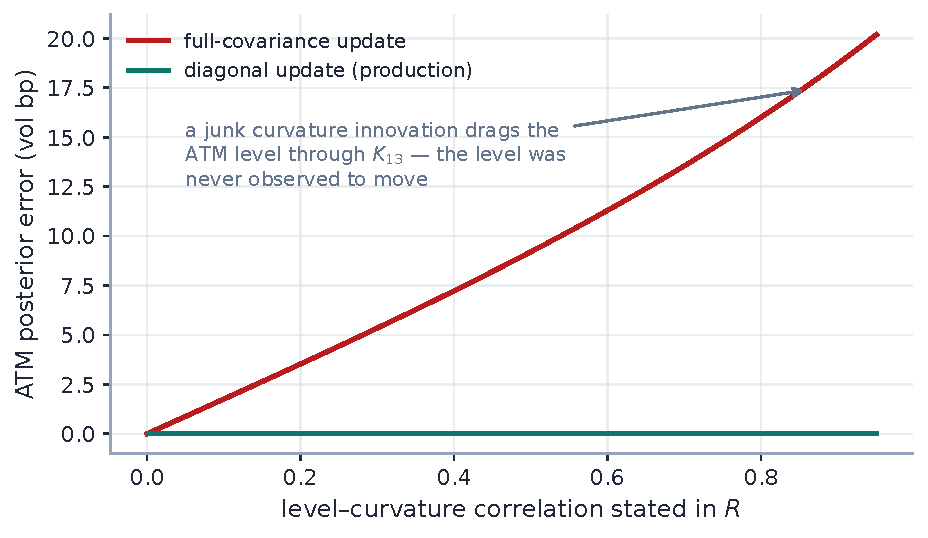
\includegraphics[width=0.86\textwidth]{fig_ktr_offdiag.pdf}
\caption{The blow-up mechanism in vitro (production update, both
paths).  A pure junk-curvature innovation is fed to the update as the
stated level--curvature correlation in $R$ rises: the full-covariance
posterior drags the ATM level by up to \ktroffdiagdrag\ vol bp ---
the level was never observed to move --- while the production
diagonalized update is immune by construction.  The real incident, with
correlated prediction uncertainty as well, reached
\ktrblowupminpts--\ktrblowupmaxpts\ vol \emph{points}.}
\label{fig:offdiag}
\end{figure}

%======================================================================
\section{Fitting under computed trust: the active MAP}
\label{sec:map}

Production ships three modes.  \texttt{off} is byte-identical to the
feature never existing.  \texttt{overlay} computes and displays ---
prediction, observation, innovation, gain, posterior, and a drawable
filtered curve with a credible band that is the functional pushforward
of the full $3\times3$ state covariance through the slice map --- but
never steers a fit; it is the sandbox in which every budget of
\cref{sec:robs,sec:pbudget} was tuned.  \texttt{active} moves the same
accounting \emph{inside} the calibration.

The wrong way to do that is to build the posterior from today's quotes
and then add it as a prior while fitting the same quotes again --- the
same information counted twice.  The correct active objective is the
one-stage MAP problem
\begin{equation}
\calL_{\mathrm{active}}(\theta)
=\calL_{\mathrm{quote}}(\theta;q_t)
+\half\norm[\big]{\calH(\theta)-m_t^-}_{(P_t^-)^{-1}}^2
+\calL_{\mathrm{intrinsic}}(\theta)
+\calL_{\mathrm{persist},\perp}(\theta),
\label{eq:active-map}
\end{equation}
today's quote likelihood plus the Kalman prediction prior plus the
intrinsic regularization plus only the persistence terms orthogonal to
the filter state.

\begin{proposition}[No double counting in the MAP form]
\label{prop:nodouble}
If the model is linear, $z=Hx+\epsilon$ with
$\epsilon\sim\mathcal N(0,R)$, and $x\sim\mathcal N(m^-,P^-)$, the
minimizer of
$\half\norm{z-Hx}_{R^{-1}}^2+\half\norm{x-m^-}_{(P^-)^{-1}}^2$
is the Kalman posterior mean of \cref{eq:kalman}, and the posterior
information is the sum $H\T R^{-1}H+(P^-)^{-1}$.
\end{proposition}

\begin{proof}
The normal equations read
$\big(H\T R^{-1}H+(P^-)^{-1}\big)x=H\T R^{-1}z+(P^-)^{-1}m^-$.
Woodbury rewrites the left inverse as
$P^--P^-H\T(HP^-H\T+R)^{-1}HP^-$; substitution gives
$x=m^-+P^-H\T(HP^-H\T+R)^{-1}(z-Hm^-)$.
\end{proof}

Production realizes \cref{eq:active-map} with four locked decisions.

\begin{enumerate}[leftmargin=1.6em]
\item \textbf{The prediction prior is an ungated operator target.}  It
reuses the smile-factor stencil legs at $k\in\{-b,0,b\}$ with $b=0.06$:
on a locally quadratic smile the identities
$\sigma(b)-\sigma(-b)=2b\,s$ and
$\sigma(b)-2\sigma(0)+\sigma(-b)=b^2\kappa$ are \emph{exact}, so the
handle targets convert to stencil targets with no approximation beyond
local quadraticity, and the prior flows to LQD, SVI and Multi-Core
Sigmoid through the existing operator plumbing with zero per-model
wiring.  Crucially it carries \emph{no} activation gate: the Kalman
prior is always on at its covariance weight --- precisely the
persistence/filter distinction of \cref{sec:dial}.
\item \textbf{The weights are the MAP objective in the fit's own
units.}  The quote rows are near-unit-weighted vol errors --- the true
MAP objective multiplied through by $s_q^2$ --- so the consistent prior
weight is $\lambda_j=s_q^2/\Var(O_j)$ with $s_q$ the node's median
stated half-spread (the same $s_q$ as \cref{sec:units}).
\item \textbf{Persistence auto-exclusion is hard-coded.}  In active
mode the resolver drops every persistence builder overlapping the
handle coordinates --- operators, smile factors, the near-ATM strike
anchor.  What survives is exactly what the filter state does not carry:
the deep-tail strike anchor and the graph's dark-node baseline.  There
is deliberately no knob; two anchors to the same previous state would
violate invariant~2.
\item \textbf{No second update.}  The committed fit \emph{is} the
one-stage MAP solution: $m^+$ is its backbone handles, and $P^+$ comes
from unwhitening the full solver information (data rows plus whitened
prior rows) by the same $s_q$ --- landing exactly at
$\calI_{\mathrm{data}}+(P^-)^{-1}$, the posterior information of
\cref{prop:nodouble}.  The MAP-equals-Kalman identity is test-locked to
$10^{-10}$.  One guard on top: $P^+$ is capped at $P^-$ per handle,
because information only adds --- inconsistent data ($\rho>1$) should
drive $P^+$ \emph{toward} the prediction uncertainty, never beyond it.
\end{enumerate}

\subsection{Opening the gate before the fit exists}
\label{sec:probegate}

The adaptive gate of \cref{sec:adaptive} reads today's innovation ---
which, on the active path, does not exist until the MAP fit has run,
and by then the prior weight is already spent.  This gap was the v2
sweep's one measured weakness (\ktractshockspike--\ktractshockhigh\ bp
of shock lag in the spike and high-vol regimes,
\cref{sec:audit}), and the shipped fix prices surprise \emph{before}
fitting: the \emph{level} row is gated by a fit-free ATM probe --- the
prepared mid IV interpolated at $k=0$, probe noise $s_q$ --- and the
\emph{shape} rows by the previous step's realized innovation, a
one-step-lagged fading memory (after a surprise day, the next prior is
wide).  The factors are deterministic in (previous state, prepared
chain, options), so the prior builder and the posterior bookkeeping
compute identical inflation and the MAP algebra stays consistent.  The
mechanism is unit-locked (the probe fires on a five-point jump in the
prepared mids; clean days are byte-identical; the gate off is the
identity).  One honesty note for the audit trail: the harness's
synthetic shock perturbs only the thinned fit inputs, \emph{not} the
prepared mids the probe reads, so the scenario A/B under-reports this
fix by construction --- the real-world path, a shock present in the
prepared chain, is the unit-tested one, and the full-regime validation
rides the next sweep.

\subsection{Where persistence remains}

Prior persistence keeps three jobs in active mode, each outside the
filter state: deep tails and operator baskets the handles do not
represent; the saved prior from which the first filtered state is
seeded; and dark graph nodes with no current observation at all.  What
it never does again is anchor ATM, skew or curvature to the same
previous state that already enters as $m^-$ --- the auto-exclusion
makes that structural rather than procedural.

\paragraph{Exercise 2.}
From \cref{prop:nodouble}, show the posterior information in the MAP
form is $\calI_{\mathrm{data}}+(P^-)^{-1}$, and conclude
$P^+\preceq P^-$ \emph{exactly} whenever the algebra is exact.  The
production per-handle cap on $P^+$ therefore only ever binds when the
finite-difference handle map or the $\rho$ inflation perturbs the
unwhitened information --- it is a numerical fence around a theorem,
not a new modelling assumption.

%======================================================================
\section{The audit: were the error bars true?}
\label{sec:audit}

A filter can always make charts smoother; the question worth money is
whether its \emph{stated uncertainty} is true.  The acceptance metric
of the temporal harness is therefore not an RMS but a calibration
statistic: the standardized residual
\[
\zeta=\frac{\text{truth}-m^+}{\sqrt{P^++R_{\mathrm{truth}}}},
\]
whose standard deviation should be $1$ if the error bars mean what they
say.  Even here honesty bites: the held-out ``truth'' is itself a
fitted estimate, and scoring against $\sqrt{P^+}$ alone overstated
miscalibration threefold before $R_{\mathrm{truth}}$ was added.  The
harness drives the \emph{production} commit path over consecutive
captured day pairs in three regimes (August 2024 spike, October 2022
high-vol, July 2023 low-vol), eight assets each: fit day $T{-}1$ and
commit through the filter; carry the state to day $T$ with the real
snapshot $\Delta t$ and forward transport; build day $T$'s measurement
from a thinned ATM-only chain under a scenario --- \texttt{thinned}
(plain), \texttt{contradiction} (two adjacent strikes kinked opposite
ways), \texttt{shock} (a true $+5$-point jump with unchanged spreads);
score the posterior against the full-chain truth and \emph{two}
baselines (raw measurement; gain-zero prediction), bucketed by maturity.
Two sweeps: the \ktrstepstotal-step tuning sweep (overlay only) and the
\ktrstepsvtwo-step v2 sweep (overlay and active, adaptive gate on).
All numbers below are read from the stored artifacts at the decision
cell (Jacobian route, $>30$d) --- nothing re-run.

\begin{figure}[H]
\centering
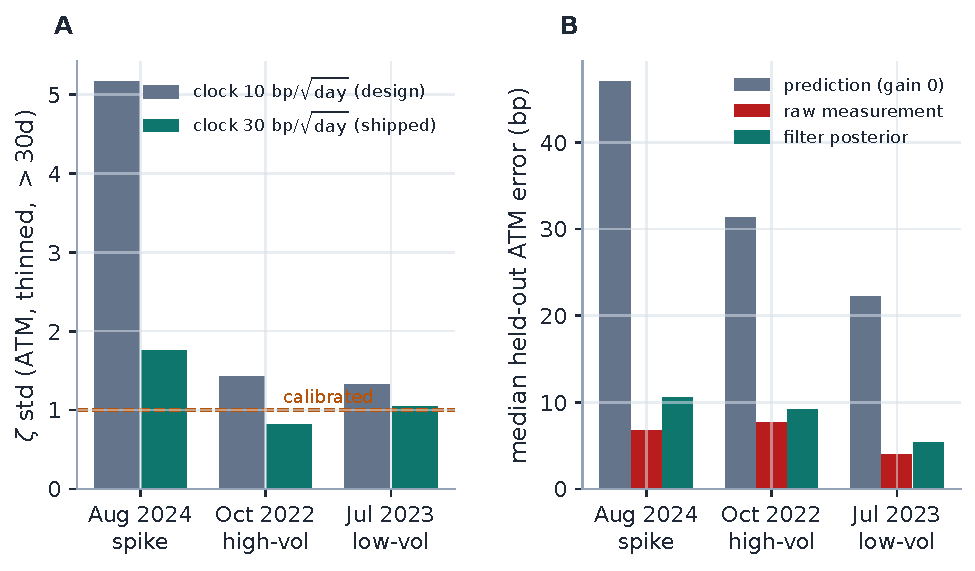
\includegraphics[width=\textwidth]{fig_ktr_backtest.pdf}
\caption{The tuning sweep's two headline panels (stored artifacts).
A: tripling the clock noise collapses the $\zeta$ std toward $1$ in
every regime
(\ktrzstdspiketen$\to$\ktrzstdspikethirty,
\ktrzstdhighten$\to$\ktrzstdhighthirty,
\ktrzstdlowten$\to$\ktrzstdlowthirty) --- the design value starved the
prediction budget, and starved budgets lie.  B: on plain thinned days
the posterior sits between the raw measurement and the gain-zero
prediction: the filter pays for itself on the noisy tail, not on clean
liquid days --- the success criterion set before the run.}
\label{fig:backtest}
\end{figure}

\paragraph{The clock default flipped ($10\to30$), for calibration
reasons.}  In every regime, on both covariance routes, at every
scenario, $q=30$ bp$/\sqrt{\text{day}}$ beats the design value of
$10$: the $\zeta$ std collapses toward $1$ (\cref{fig:backtest}A),
shock lag shrinks
\ktrshockimprovemin--\ktrshockimprovemax$\times$, win rates rise.  The
lesson generalizes: a too-small process budget does not make a filter
cautious --- it makes it \emph{overconfident and slow}, the worst pair.

\paragraph{Jacobian versus factors is a real trade-off; Jacobian stays
the default.}  On \texttt{contradiction} --- the core denoising case
--- the Jacobian route wins $2$--$3\times$ in every regime (spike
\ktrcontrajacspike\ vs \ktrcontrafacspike\ bp; high
\ktrcontrajachigh\ vs \ktrcontrafachigh; low \ktrcontrajaclow\ vs
\ktrcontrafaclow): its geometry-aware $R$ sees which directions the
kinked cluster fails to identify.  On \texttt{shock} the ranking
reverses (spike \ktrshockjacspike\ vs \ktrshockfacspike\ bp lag): the
factor route's blunter, smaller $R$ yields higher gain.  Contradiction
rejection is the feature's purpose, the shock gap closes under the
adaptive gate below, and the factor route stays one knob away.

\paragraph{The honest median-day statement.}  On plain consecutive days
the raw measurement is already good
(\ktrerrmeaslow--\ktrerrmeashigh\ bp median ATM error across regimes)
and the filter's median win rate is
\ktrwinspike--\ktrwinhigh\ --- \emph{below} one half.  The posterior
(\ktrerrpostspike/\ktrerrposthigh/\ktrerrpostlow\ bp per regime) beats
the gain-zero prediction
(\ktrerrpredspike/\ktrerrpredhigh/\ktrerrpredlow\ bp) everywhere but
does not beat a clean measurement on a clean day --- and should not:
the success criterion was ``lower held-out error on \emph{noisy}
snapshots'', never ``lower every RMS''.  Two recorded artifacts of the
harness itself: slightly negative $\zeta$ means on thinned days (the
ATM-window thinning is mildly biased against the full-chain truth), and
a $\le30$ DTE bucket that is a different regime --- $90$--$160$ bp
thinned-vs-full discrepancies from short-end quote and de-Am noise,
reported separately so neither bucket masks the other, and the reason
for the maturity noise floor of \cref{sec:robs}.

\paragraph{The adaptive gate, validated at full scale.}  The v2 sweep
turns the surprise gate on everywhere and the shock columns collapse:
\ktrshockjacspike$\,\to\,$\ktrovlshockspike\ bp in the spike regime,
\ktrshockjachigh$\,\to\,$\ktrovlshockhigh\ in high-vol,
\ktrshockjaclow$\,\to\,$\ktrovlshocklow\ in low-vol
(\cref{fig:active}B), with thinned and contradiction cells unchanged
--- the gate opens on genuine shocks and stays quiet on clean and on
contradictory days, exactly the composition \cref{sec:adaptive}
promised.

\paragraph{Active mode, measured at full scale.}  In active mode the
committed fit \emph{is} the MAP solution, so the baseline is the
overlay run's raw column of the same sweep.  The verdict is one-sided
wherever denoising is the job (\cref{fig:active}A): on plain thinned
days the active MAP beats \emph{both} the raw fit and the overlay
posterior in every regime
(\ktractthinspike/\ktractthinhigh/\ktractthinlow\ bp against raw
\ktrerrmeasspike/\ktrerrmeashigh/\ktrerrmeaslow), and on contradiction
days it wins outright in the high- and low-vol regimes
(\ktractcontrahigh\ vs \ktrrawcontrahigh\ bp raw; \ktractcontralow\ vs
\ktrrawcontralow) while in the spike regime it beats the post-hoc blend
(\ktractcontraspike\ vs \ktrovlcontraspike\ bp) though not the raw fit
(\ktrrawcontraspike\ bp) --- all with honest uncertainty ($\zeta$ std
\ktractzetamin--\ktractzetamax\ over those cells).  Fitting quotes and
prediction jointly beats blending them afterwards, exactly as
\cref{prop:nodouble} says it should.  The measured weakness is the
shock scenario
(\ktractshockspike--\ktractshockhigh\ bp lag in the spike and high-vol
regimes): the MAP prior weight was priced before the measurement
existed.  That is precisely the gap the probe-and-lag gate of
\cref{sec:probegate} closes by construction; its full-regime scorecard
is the flagged item before any active-by-default discussion.

\begin{figure}[H]
\centering
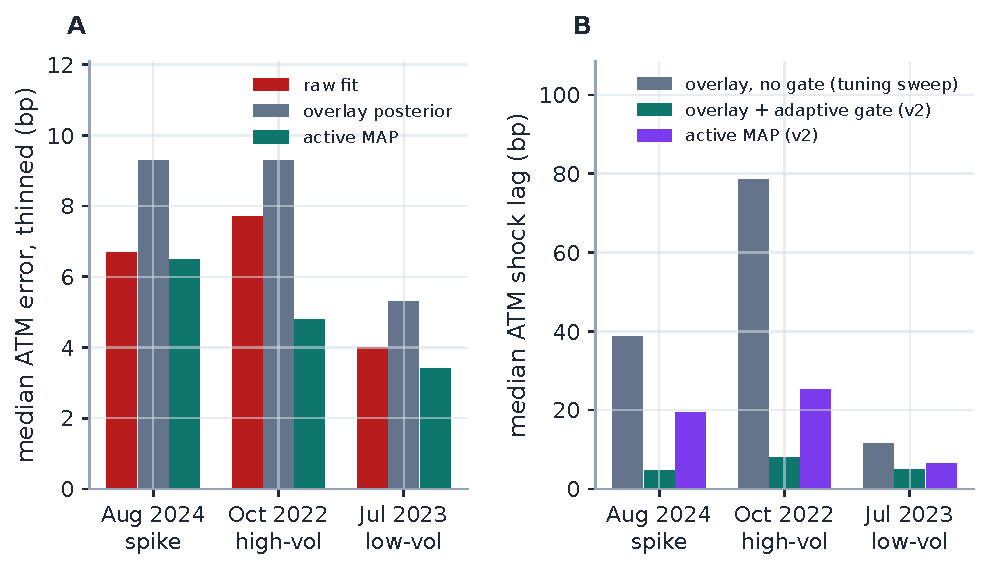
\includegraphics[width=\textwidth]{fig_ktr_active.pdf}
\caption{The v2 sweep (stored artifacts; $>30$d, Jacobian route).
A: on plain thinned days the active one-stage MAP is the best of the
three in every regime --- joint fitting beats post-hoc blending.
B: the shock columns: the un-gated tuning-sweep overlay lags badly, the
adaptive gate collapses the lag
(\ktrshockjachigh$\to$\ktrovlshockhigh\ bp in high-vol), and the active
MAP still lags --- its prior was priced before the measurement existed,
the gap the fit-path probe gate closes.}
\label{fig:active}
\end{figure}

\paragraph{Exercise 3.}
A +5-point overnight jump under a $30$ bp$/\sqrt{\text{day}}$ clock is
a ${\sim}50\sigma$ event: compute the un-gated gain for a liquid chain
($r\approx(10\,\text{bp})^2$, $p=q^2\Delta t$) and the residual lag
after one update; then apply the $(\zeta/3)^2$ inflation and recompute.
Explain why the same inflation does \emph{not} fire on the
contradiction scenario even though its innovation is also large in raw
units (the $\rho$-inflated $R$ enters the standardization).

%======================================================================
\section{What is genuinely original here}
\label{sec:original}

The equations are Kalman's \cite{Kalman1960,AndersonMoore1979}; the
contribution is a discipline.  \emph{Three notions usually blended in
volatility tools are held separate}: today's quote likelihood
(Note~07), the temporal state with prediction and measurement
covariances (this note), and gap persistence that activates only where
quotes do not identify a functional (Note~13) --- the separation is
what lets the filter denoise without using yesterday as a fake quote,
and persistence stabilize wings without damping a real move.  \emph{The
measurement covariance is a market object}: propagated from the fit's
own information in stated bid--ask units, with the eigen-clamp choosing
the honest sign of failure and the $\chi^2$ inflation converting
internal contradiction into stated noise --- so the gain falls on a
lying chain with no thresholds anywhere.  \emph{The prediction budget
runs on the market's clock}, with a measured cadence audit behind the
session clock and a surprise gate that composes correctly with the
contradiction inflation.  \emph{The active mode is an accounting
identity}, not a feature: one-stage MAP with the ungated stencil prior,
hard-coded persistence exclusion, and a posterior read off the solver's
own information --- double counting made impossible rather than
discouraged.  And the whole feature is judged by \emph{calibration of
uncertainty} ($\zeta\to1$), the audit that flipped a default, chose a
route, and convicted a matrix.

%======================================================================
\section{Limitations}
\label{sec:limits}

Where the guarantees stop.  \emph{The diagonal update discards genuine
cross-handle information}; the blow-up showed why that trade is
currently right, and a shrunk-correlation update is a live research
item, not a closed door.  \emph{The session clock is measured but not
default}: calendar remains the byte-identical default, and the
campaign's residual is real --- at the default per-handle scales the
skew and curvature $\zeta$ run $1.8$ and $6.4$ on the thirty-minute
cadence, worst on short-dated nodes, so per-maturity handle scales are
the recorded follow-up.  \emph{The fit-path surprise gate is shipped
but not yet sweep-validated}: the harness's synthetic shock cannot see
it by construction (\cref{sec:probegate}), so its evidence is
unit-level until the next full-regime run --- \emph{the} open item
before any active-by-default.  \emph{The short end stays the weakest
bucket}: the $\sqrt{30/\mathrm{DTE}}$ floor sizes $R$ honestly below
$30$ DTE, but honest uncertainty is not signal.  \emph{The state is
per-node}: a graph-coupled filter (Note~14's block covariance with
time dynamics) is deferred until the single-node filter has earned
trust.  And \emph{the measurement carrier is the LQD backbone}: a
displayed model whose handles disagree with the backbone's inherits
that disagreement through the overlay.

\appendix
%======================================================================
\section{Hyperparameter atlas}
\label{app:atlas}

The only home for settings names: the body speaks mathematics, this
table speaks configuration.

\begingroup
\small
\begin{longtable}{p{0.34\textwidth}p{0.13\textwidth}p{0.45\textwidth}}
\caption{Observation-filter hyperparameters, as shipped.}\label{tab:atlas}\\
\toprule Knob & Default & Role\\ \midrule
\endfirsthead \toprule Knob & Default & Role\\ \midrule \endhead
\multicolumn{3}{l}{\emph{Surfaced (options settings)}}\\ \midrule
\texttt{observationFilterMode} & \texttt{off} & \texttt{off} /
\texttt{overlay} / \texttt{active} (\cref{sec:map}); \texttt{off} is
byte-identical to the feature never existing.\\
\texttt{filterCovarianceMode} & \texttt{jacobian} & Measurement route:
\cref{eq:cov-delta} (backtested default) or \cref{eq:cheapR} (fallback
+ A/B column).\\
\texttt{filterProcessVolBpSqrtDay} & $30$ & ATM clock noise (vol bp per
$\sqrt{\text{day}}$); flipped from the design $10$ by the audit
(\cref{fig:backtest}A).\\
\texttt{filterProcessSkewSqrtDay} & $0.02$ & Skew clock scale.\\
\texttt{filterProcessCurvSqrtDay} & $0.05$ & Curvature clock scale.\\
\texttt{filterTransportNoiseScale} & $0.10$ & Extra process std per unit
$\abs h$ transport distance.\\
\texttt{filterResidualInflation} & on & Apply
\cref{eq:resid-inflation}.\\
\texttt{filterAdaptiveSigma} & $3$ & Surprise gate
(\cref{sec:adaptive}); overlay gates on today's innovation, active on
the ATM probe + lagged innovation (\cref{sec:probegate}); $0$ = off.\\
\texttt{filterMaxGain} & $1.0$ & Pilot own-gain cap; never binds at
$1.0$.\\
\texttt{filterResetHours} & $96$ & Maximum gap predicted across; longer
resets as \texttt{stale} (spans a weekend plus a holiday).\\
\texttt{filterClock} & \texttt{calendar} & Process-noise clock:
\texttt{calendar} (wall-clock days, byte-identical legacy) or
\texttt{session} (the intraday variance clock, \cref{sec:clock}).
Resets stay on calendar hours regardless.\\
\texttt{filterSessionShare} & $0.60$ & Share of a day's variance
accrued in the exchange session under the session clock.\\
\texttt{filterNonTradingWeight} & $0.0$ & A closed day's variance
weight under the session clock (a weekend $\approx$ one overnight,
measured).\\
\texttt{filterDataOnlyPrepass} & off & Opt-in extra data-only fit so
$z_t$ is strictly persistence-free; off flags contamination instead.\\
\midrule
\multicolumn{3}{l}{\emph{Hidden (internal constants)}}\\ \midrule
\texttt{DIAGONAL\_UPDATE} & on & Per-handle scalar gains
(\cref{sec:matrix}); the measured answer to the off-diagonal blow-up.\\
\texttt{FILTER\_STENCIL\_H} & $0.06$ & ATM stencil half-width of the
active MAP prior legs (exact identities on a locally quadratic
smile).\\
\texttt{RESID\_INFLATION\_CAP} & $25$ & Cap on $\rho$ and on the
adaptive inflation factors: one broken chain cannot poison the state.\\
\texttt{SHORT\_DATED\_REF\_DAYS} & $30$ & Noise floor
$\sqrt{30/\mathrm{DTE}}$ below $30$ DTE, applied to $R_t$, the MAP
weights and the unwhitening.\\
\texttt{INFO\_RANK\_RTOL} & $10^{-10}$ & Eigen-clamp cutoff of
$\calI_\theta$: small eigenvalues clamp \emph{up}, so unidentified
directions inflate $R$ finitely (\cref{sec:units}).\\
\texttt{CHOL\_JITTER} & $10^{-12}$ & Whitening-Cholesky base jitter;
any nonzero use is a reported diagnostic event, never silent.\\
\texttt{HANDLE\_MOVE\_SCALES} & $(0.03,0.05,0.5)$ & Typical one-day
move scales (the Note~14 units convention) sizing the transport term.\\
\texttt{RMS\_FLOOR} & $10^{-4}$ & Floor on the stated per-quote noise
(one vol bp); chains without band data use $10\times$ this floor.\\
variance envelope & graph floors/caps & Per-handle $R$ diagonals
clipped into the graph layer's sanity envelope, correlations rescaled
to survive.\\
\texttt{\_filter\_version} & --- & Overlay-only knob changes bump a
lightweight version (no fit-cache invalidation); only
\texttt{active}-affecting changes bump the options version.\\
\bottomrule
\end{longtable}
\endgroup

%======================================================================
\section{Performance notes}
\label{app:perf}

\begin{enumerate}[leftmargin=1.6em]
\item \textbf{Overlay mode is invisible next to calibration}: a dense
$d\times d$ solve with $d=3$, state storage $O(d^2)$ per node.
\item \textbf{The Jacobian covariance is nearly free}: $J\T WJ$ comes
from the solution Jacobian the calibrators already retain, and $G$ is
$2P$ slice \emph{builds} on the coarse optimization grid --- about
$4\times$ cheaper per build than the display quadrature.
\item \textbf{Seeding must never hide a fit.}  The first implementation
seeded through the prior bootstrap branch, whose fetch path silently ran
a full extra mid calibration per node --- switching the filter on made a
live universe crawl.  The shipped rule seeds from the transported saved
prior, else from the committed fit's own handles at bootstrap-tier
precision: the same information, for free.  Reverted-and-redesigned,
per house practice.
\item \textbf{Overlay curves are memoized per committed state.}  The
filtered curve is the backbone retargeted to $m^+$ (a Newton solve,
Note~01) plus the functional band; computing them per GET made the live
UI feel frozen, since the smile view polls per refresh signal.
\item \textbf{Active MAP adds no second fit pass}: three residual rows
in the existing stack; the data-only prepass is the only real cost
lever and is off by default.
\item \textbf{The session clock costs an integral over day segments},
microseconds per prediction; the cadence audit itself
(\cref{fig:clock}) reads stored campaign tables.  No benchmark in this
note was re-timed; figures and macros were generated at commit
\texttt{\ktrgencommit} on \ktrgendate.
\end{enumerate}

%======================================================================
\section{Traceability}
\label{app:trace}

\begingroup
\small
\setlength{\tabcolsep}{3pt}
\begin{longtable}{@{}p{0.34\textwidth}p{0.14\textwidth}p{0.24\textwidth}p{0.22\textwidth}@{}}
\caption{Claims in this note and the code/tests that lock them.}\\
\toprule Claim & Object & Code anchor & Test anchor\\ \midrule
\endfirsthead
\toprule Claim & Object & Code anchor & Test anchor\\ \midrule
\endhead
Joseph update PSD for any gain; own-gain cap; scalar shrinkage; agrees
with the graph posterior to $10^{-12}$ &
\cref{eq:kalman}, \cref{prop:scalar} &
\nolinkurl{calib/observation_filter.py} &
\nolinkurl{test_observation_filter.py}\\
One-stage MAP minimizer $=$ Kalman posterior to $10^{-10}$; ungated
stencil prior; no second update &
\cref{prop:nodouble}, \cref{eq:active-map} &
\nolinkurl{calib/observation_filter.py},
\nolinkurl{api/observation_filter.py} &
\nolinkurl{test_observation_filter.py},
\nolinkurl{test_filter_active.py}\\
Jacobian covariance; regularized eigen-inverse; stated-noise units
contract &
\cref{eq:cov-delta}, \cref{sec:units} &
\nolinkurl{calib/observation_measurement.py} &
\nolinkurl{test_observation_measurement.py}\\
Contradictions inflate $R$; band rows contribute nothing inside the
spread &
\cref{eq:resid-inflation} &
\nolinkurl{calib/observation_measurement.py} &
\nolinkurl{test_observation_measurement.py}\\
Diagonal update; idempotent commits; reset matrix; seeding without a
hidden fit; short-dated floor &
\cref{sec:matrix}, \cref{sec:lifecycle} &
\nolinkurl{api/observation_filter.py} &
\nolinkurl{test_observation_filter_app.py}\\
Mode resolution; \texttt{off} byte-identical; overlay never steers
fits &
\cref{sec:map} &
\nolinkurl{api/filter_mode.py} &
\nolinkurl{test_filter_mode.py}\\
Persistence auto-exclusion: only the deep-tail anchor and dark nodes
survive in active mode &
\cref{sec:map} &
\nolinkurl{api/prior_mode.py} &
\nolinkurl{test_filter_active.py::test_auto_exclusion_truth_table}\\
Active-path surprise gate: ATM probe + lagged shape gate, deterministic
factors &
\cref{sec:probegate} &
\nolinkurl{api/observation_filter.py} &
\nolinkurl{test_observation_filter_app.py::test_active_adaptive_probe_and_lag}\\
Session clock: nests the calendar convention; shapes the filter
$\Delta t$; resets stay on calendar hours &
\cref{sec:clock} &
\nolinkurl{calib/intraday_time.py},
\nolinkurl{api/observation_filter.py} &
\nolinkurl{test_intraday_time.py},
\nolinkurl{test_observation_filter_app.py::test_filter_dt_days_session_clock_shapes}\\
Temporal backtest protocol, scenarios and $\zeta$ scoring &
\cref{sec:audit} &
\nolinkurl{backtest/observation_filter.py} &
\nolinkurl{test_filter_backtest.py}\\
0DTE cadence campaign (measurement tables and clock sweep) &
\cref{sec:clock} &
\nolinkurl{backtest/observation_filter_intraday.py} &
\nolinkurl{test_intraday_time.py}\\
\bottomrule
\end{longtable}
\endgroup

%======================================================================
\section{Reference implementation}
\label{app:ref}

The numerical heart is small and model-free.  Executed against the
production \texttt{kalman\_update} on a random-seeded $3\times3$ problem
(full covariances, $H=I$), and against the production whitened MAP rows
and prior-weight identity, the maximum deviation across mean,
covariance, innovation, innovation covariance, gain, whitening and
$\lambda_j=s_q^2/\Var(O_j)$ is at most \ktrrefagree\ --- machine
precision, as it should be: production adds only input validation, the
own-gain cap and the PSD guard around the same algebra.

\begin{lstlisting}[caption={Covariance-form update with Joseph
covariance (verified against production; agreement stated above).}]
def kalman_update_ref(mean_pred, cov_pred, obs, obs_cov, H=None):
    m = np.asarray(mean_pred, dtype=float)
    P = np.asarray(cov_pred, dtype=float)
    z = np.asarray(obs, dtype=float)
    R = np.asarray(obs_cov, dtype=float)
    H = np.eye(m.size) if H is None else np.asarray(H, dtype=float)
    innovation = z - H @ m
    S = H @ P @ H.T + R
    K = np.linalg.solve(S.T, (P @ H.T).T).T
    out_mean = m + K @ innovation
    I_KH = np.eye(m.size) - K @ H
    out_cov = I_KH @ P @ I_KH.T + K @ R @ K.T
    return out_mean, 0.5 * (out_cov + out_cov.T), innovation, S, K
\end{lstlisting}

\begin{lstlisting}[caption={Whitened residual rows for the active MAP
prediction prior (distilled from
\texttt{calib/observation\_filter.py}; production escalates a reported
jitter --- a diagnostic event, never a silent repair).}]
def prediction_prior_residual(model_handles, mean_pred, cov_pred):
    L = np.linalg.cholesky(np.asarray(cov_pred, dtype=float))
    return np.linalg.solve(L, np.asarray(model_handles) - np.asarray(mean_pred))
\end{lstlisting}

\begin{thebibliography}{9}
\bibitem{Kalman1960} R.~E.~Kalman. A new approach to linear filtering
and prediction problems. \emph{Journal of Basic Engineering},
82(1):35--45, 1960.
\bibitem{AndersonMoore1979} B.~D.~O.~Anderson and J.~B.~Moore.
\emph{Optimal Filtering}. Prentice-Hall, 1979.
\bibitem{Gelman2013} A.~Gelman et al. \emph{Bayesian Data Analysis}.
CRC Press, 3rd ed., 2013.
\bibitem{Gatheral2006} J.~Gatheral. \emph{The Volatility Surface}.
Wiley, 2006.
\end{thebibliography}

\end{document}
